% region zapojeniA

\begin{figure}[h!]
    \centering
    \includegraphics[width=0.8\textwidth]{microcap/AKO/1-100kR.png}
    \caption{Zapojení a) OZ 1458 -- Časová závislost napětí v různých bodech obvodu, nejdůležitější je výstup zapojení (červeně) a napětí na kondenzátoru (zeleně), \(R_{p} =\qty{100}{\kilo\ohm}\) . Dále vidíme hysterezní smyčku komparátoru.}
    \label{fig:microcap/AKO/1-100kR.png}
\end{figure}

\begin{figure}[h!]
    \centering
    \includegraphics[width=0.8\textwidth]{microcap/AKO/2-0R.png}
    \caption{Zapojení a) OZ 1458 -- Stejně jako v Obr. \ref{fig:microcap/AKO/1-100kR.png}, jen pro \(R_{p} =\qty{0}{\ohm}\). Zde je již patrné zkosení hran dané mezní rychlostí přeběhu.}
    \label{fig:microcap/AKO/2-0R.png}
\end{figure}

\begin{figure}[h!]
    \centering
    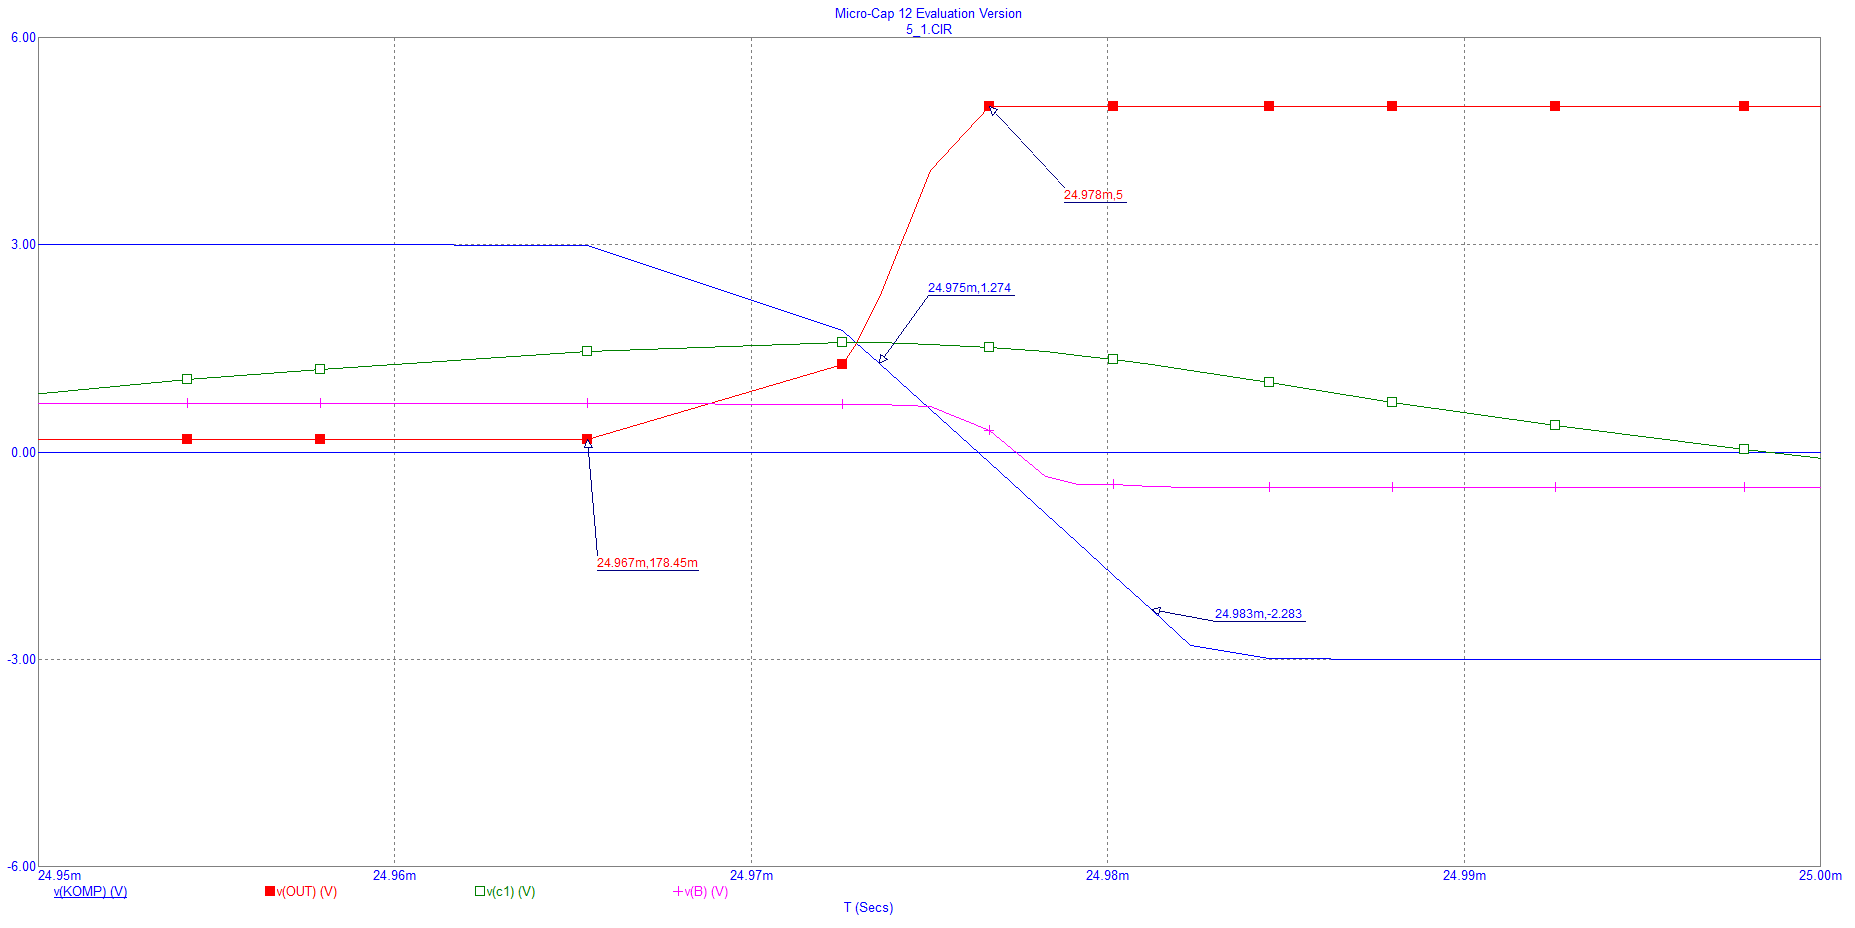
\includegraphics[width=0.8\textwidth]{microcap/AKO/3-strmost0R.png}
    \caption{Zapojení a) OZ 1458 -- Detail náběžné hrany výstupního signálu (červeně) a sestupné hrany signálu na komparátoru (modře).}
    \label{fig:microcap/AKO/3-strmost0R.png}
\end{figure}

\begin{figure}[h!]
    \centering
    \includegraphics[width=0.8\textwidth]{microcap/AKO/4-100k-071.png}
    \caption{Zapojení a) OZ 072 -- Časová závislost napětí v různých bodech obvodu, nejdůležitější je výstup zapojení (červeně) a napětí na kondenzátoru (zeleně), \(R_{p} =\qty{100}{\kilo\ohm}\) . Dále vidíme hysterezní smyčku komparátoru.}
    \label{fig:microcap/AKO/4-100k-071.png}
\end{figure}

\begin{figure}[h!]
    \centering
    \includegraphics[width=0.8\textwidth]{microcap/AKO/5-0R-071.png}
    \caption{Zapojení a) OZ 072 -- Stejně jako v Obr. \ref{fig:microcap/AKO/4-100k-071.png}, jen pro \(R_{p} =\qty{0}{\ohm}\). Zkosení hran je méně výrazné než u OZ 1458, z důvodu lepší hodnoty SR u OZ 072.}
    \label{fig:microcap/AKO/5-0R-071.png}
\end{figure}

\begin{figure}[h!]
    \centering
    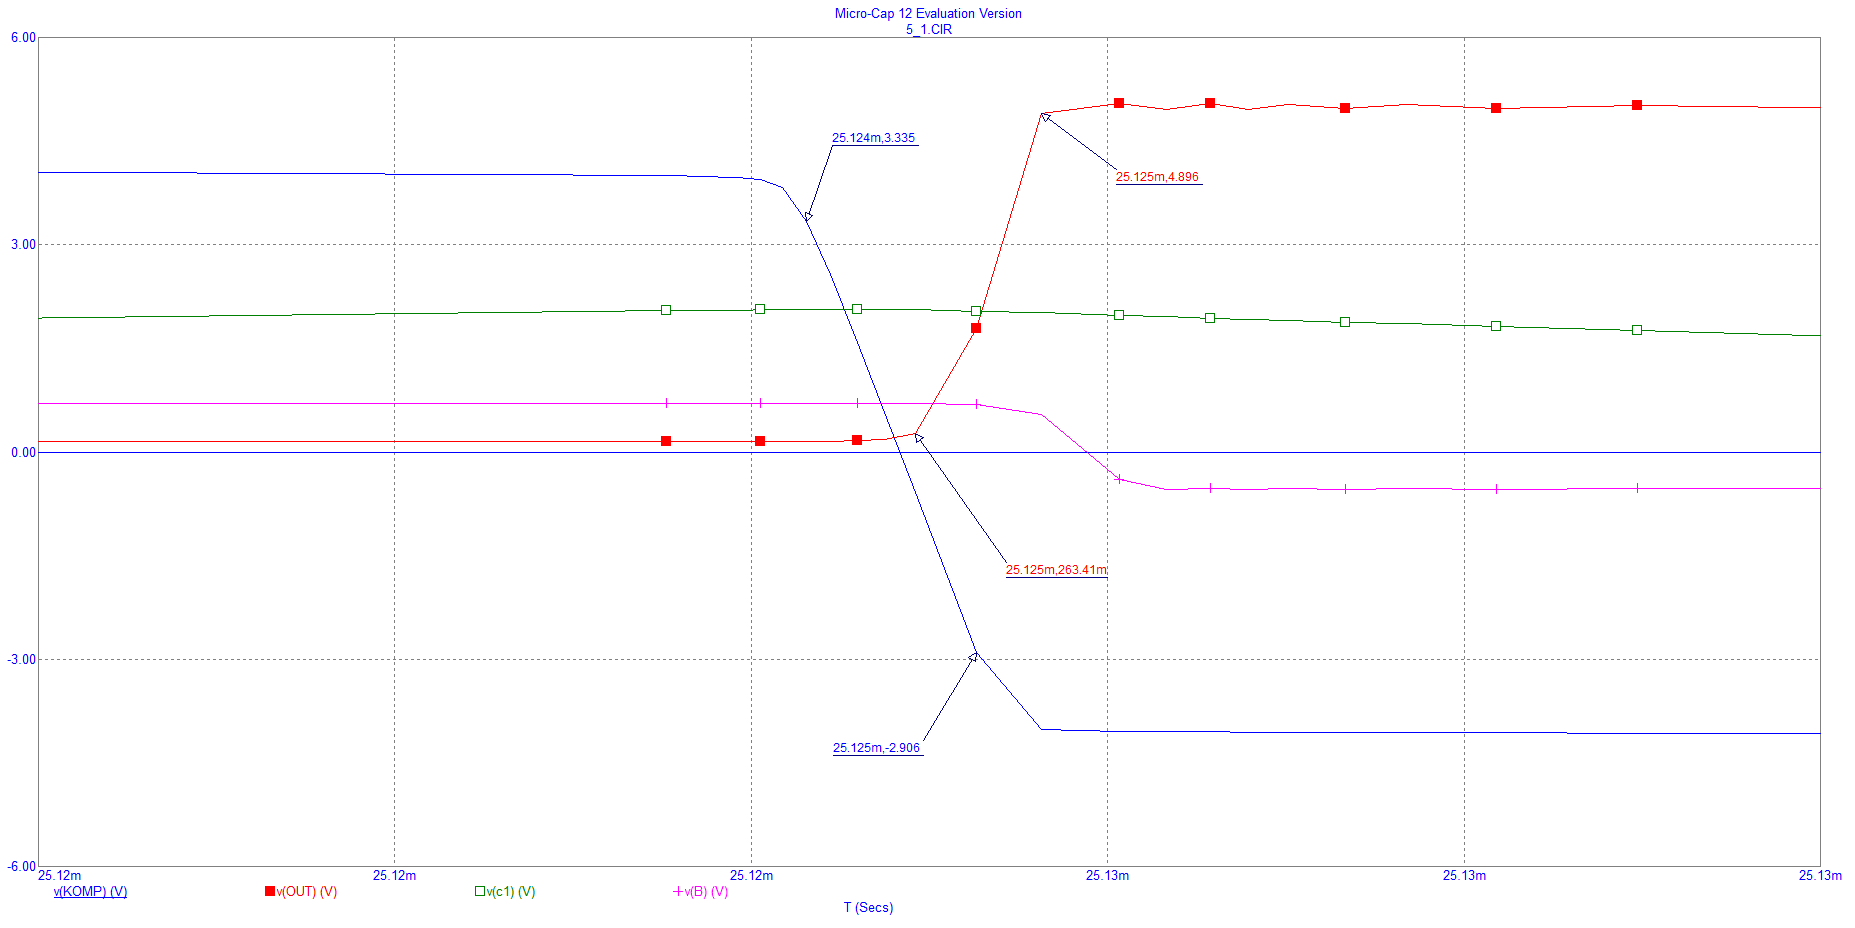
\includegraphics[width=0.8\textwidth]{microcap/AKO/6-strmost0R-071.png}
    \caption{Zapojení a) OZ 072 -- Detail náběžné hrany výstupního signálu (červeně) a sestupné hrany signálu na komparátoru (modře).}
    \label{fig:microcap/AKO/6-strmost0R-071.png}
\end{figure}

% endregion


% region zapojeniB
\begin{figure}[h!]
    \centering
    \includegraphics[width=0.8\textwidth]{microcap/AKO2/1-100kR.png}
    \caption{Zapojení b) OZ 1458 -- Časová závislost napětí na výstupu prvního OZ (obdélník) a druhého OZ (pila), \(R_{p} =\qty{100}{\kilo\ohm}\) . Dále vidíme hysterezní smyčku komparátoru.}
    \label{fig:microcap/AKO2/1-100kR.png}
\end{figure}

\begin{figure}[h!]
    \centering
    \includegraphics[width=0.8\textwidth]{microcap/AKO2/2-0R.png}
    \caption{Zapojení b) OZ 1458 -- Stejně jako v Obr. \ref{fig:microcap/AKO2/1-100kR.png}, jen pro \(R_{p} =\qty{0}{\ohm}\). Opět je zde patrné zkosení hran dané mezní rychlostí přeběhu.}
    \label{fig:microcap/AKO2/2-0R.png}
\end{figure}

\begin{figure}[h!]
    \centering
    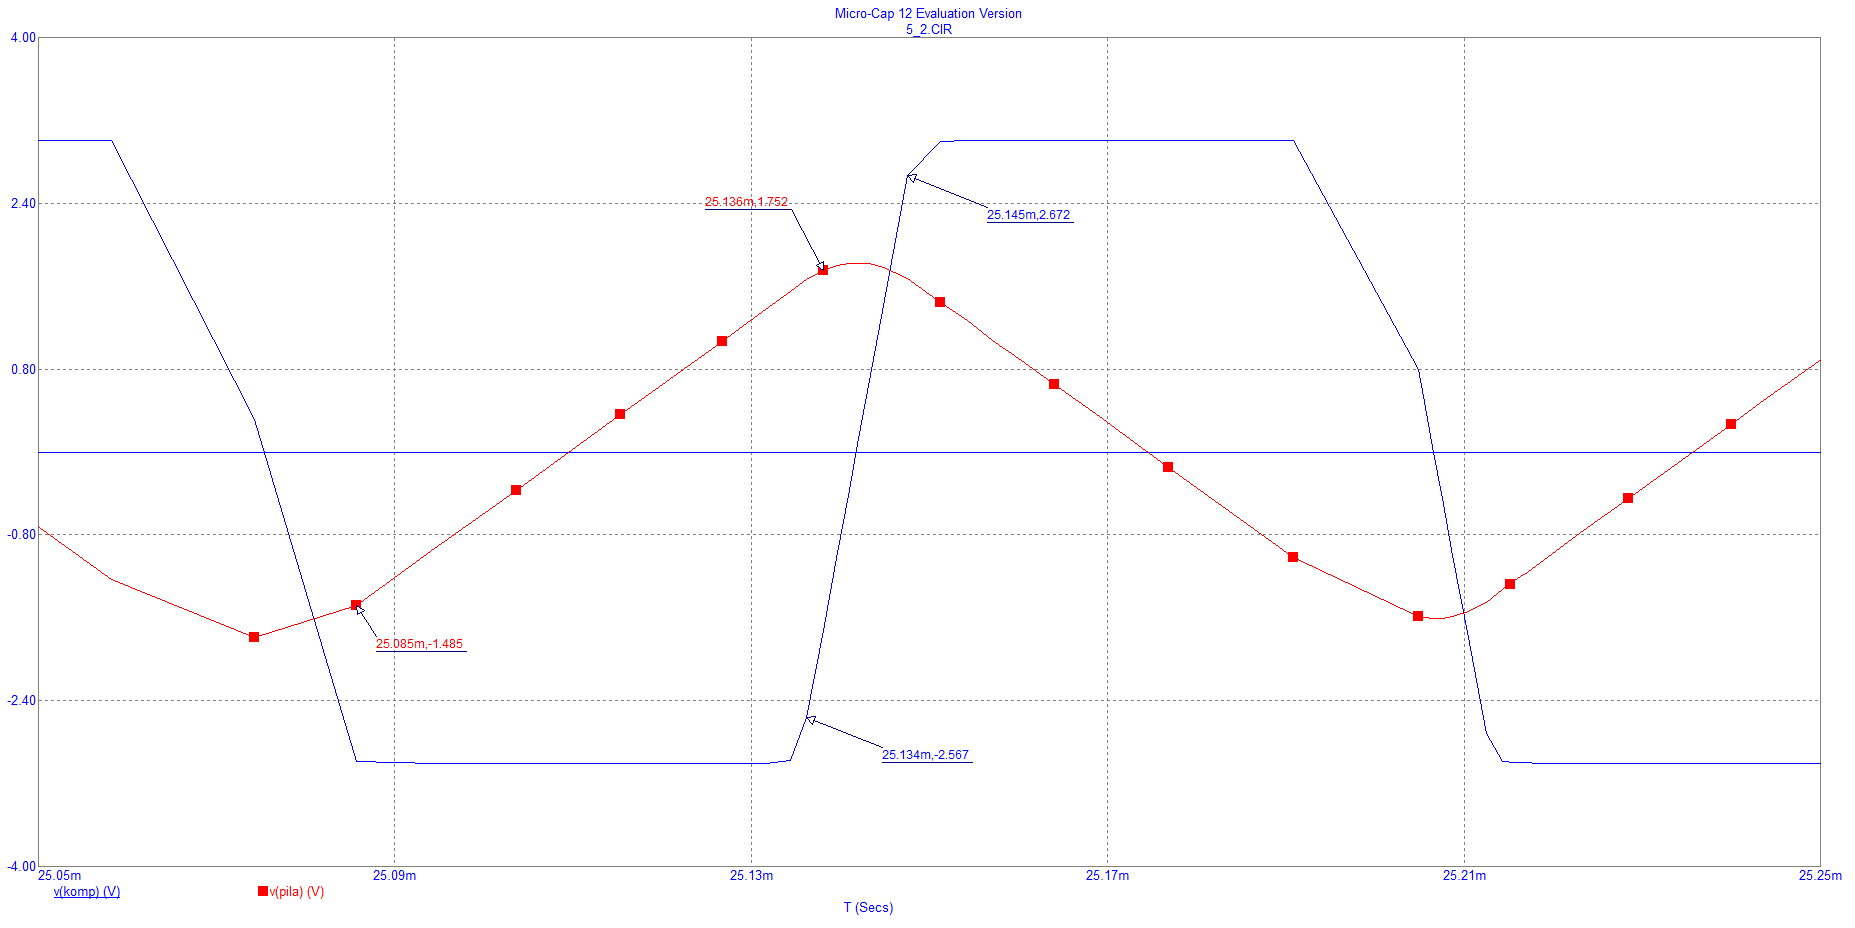
\includegraphics[width=0.8\textwidth]{microcap/AKO2/3-0R-strmost.png}
    \caption{Zapojení b) OZ 1458 -- Detail náběžné hrany signálu na výstupu prvního OZ (modře).}
    \label{fig:microcap/AKO2/3-0R-strmost.png}
\end{figure}

\begin{figure}[h!]
    \centering
    \includegraphics[width=0.8\textwidth]{microcap/AKO2/4-100k-071.png}
    \caption{Zapojení b) OZ 072 -- Časová závislost napětí na výstupu prvního OZ (obdélník) a druhého OZ (pila), \(R_{p} =\qty{100}{\kilo\ohm}\) . Dále vidíme hysterezní smyčku komparátoru.}
    \label{fig:microcap/AKO2/4-100k-071.png}
\end{figure}

\begin{figure}[h!]
    \centering
    \includegraphics[width=0.8\textwidth]{microcap/AKO2/5-0R-071.png}
    \caption{Zapojení b) OZ 072 -- Stejně jako v Obr. \ref{fig:microcap/AKO2/4-100k-071.png}, jen pro \(R_{p} =\qty{0}{\ohm}\). Zkosení hran je minimální.}
    \label{fig:microcap/AKO2/5-0R-071.png}
\end{figure}

\begin{figure}[h!]
    \centering
    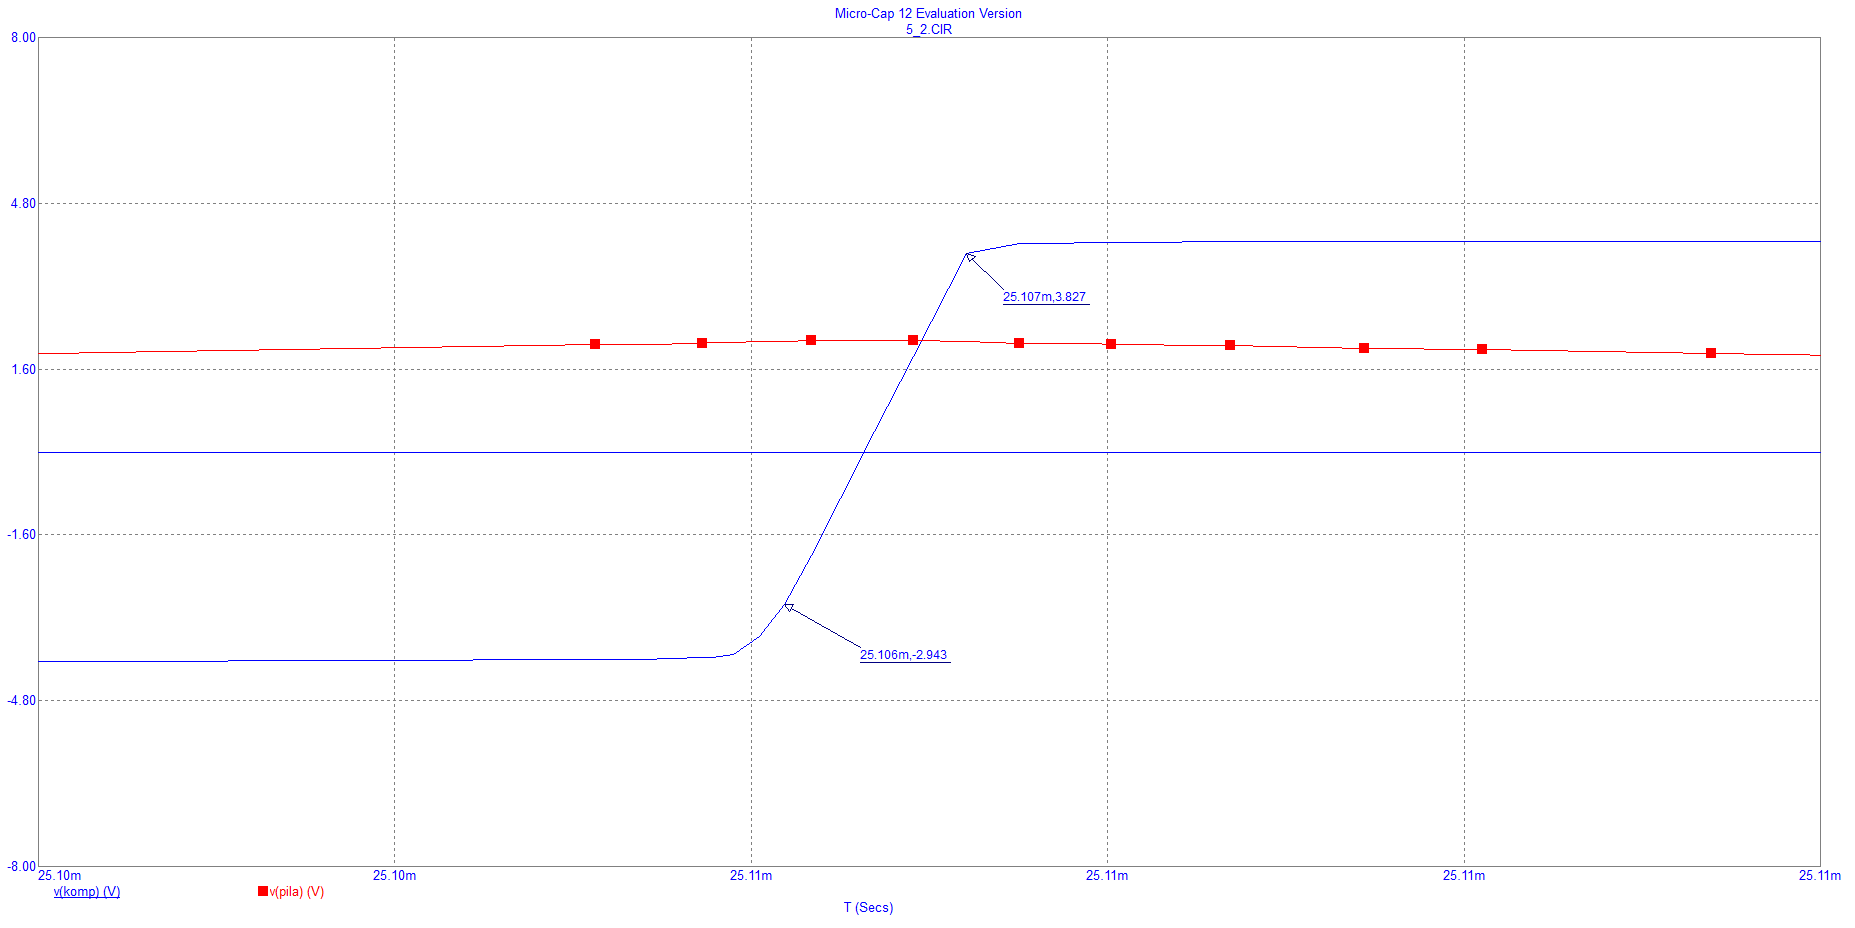
\includegraphics[width=0.8\textwidth]{microcap/AKO2/6-0R-071-strmost.png}
    \caption{Zapojení b) OZ 072 -- Detail náběžné hrany na výstupu prvního OZ.}
    \label{fig:microcap/AKO2/6-0R-071-strmost.png}
\end{figure}

% endregion
